\begin{figure}[htbp]

\begin{center}
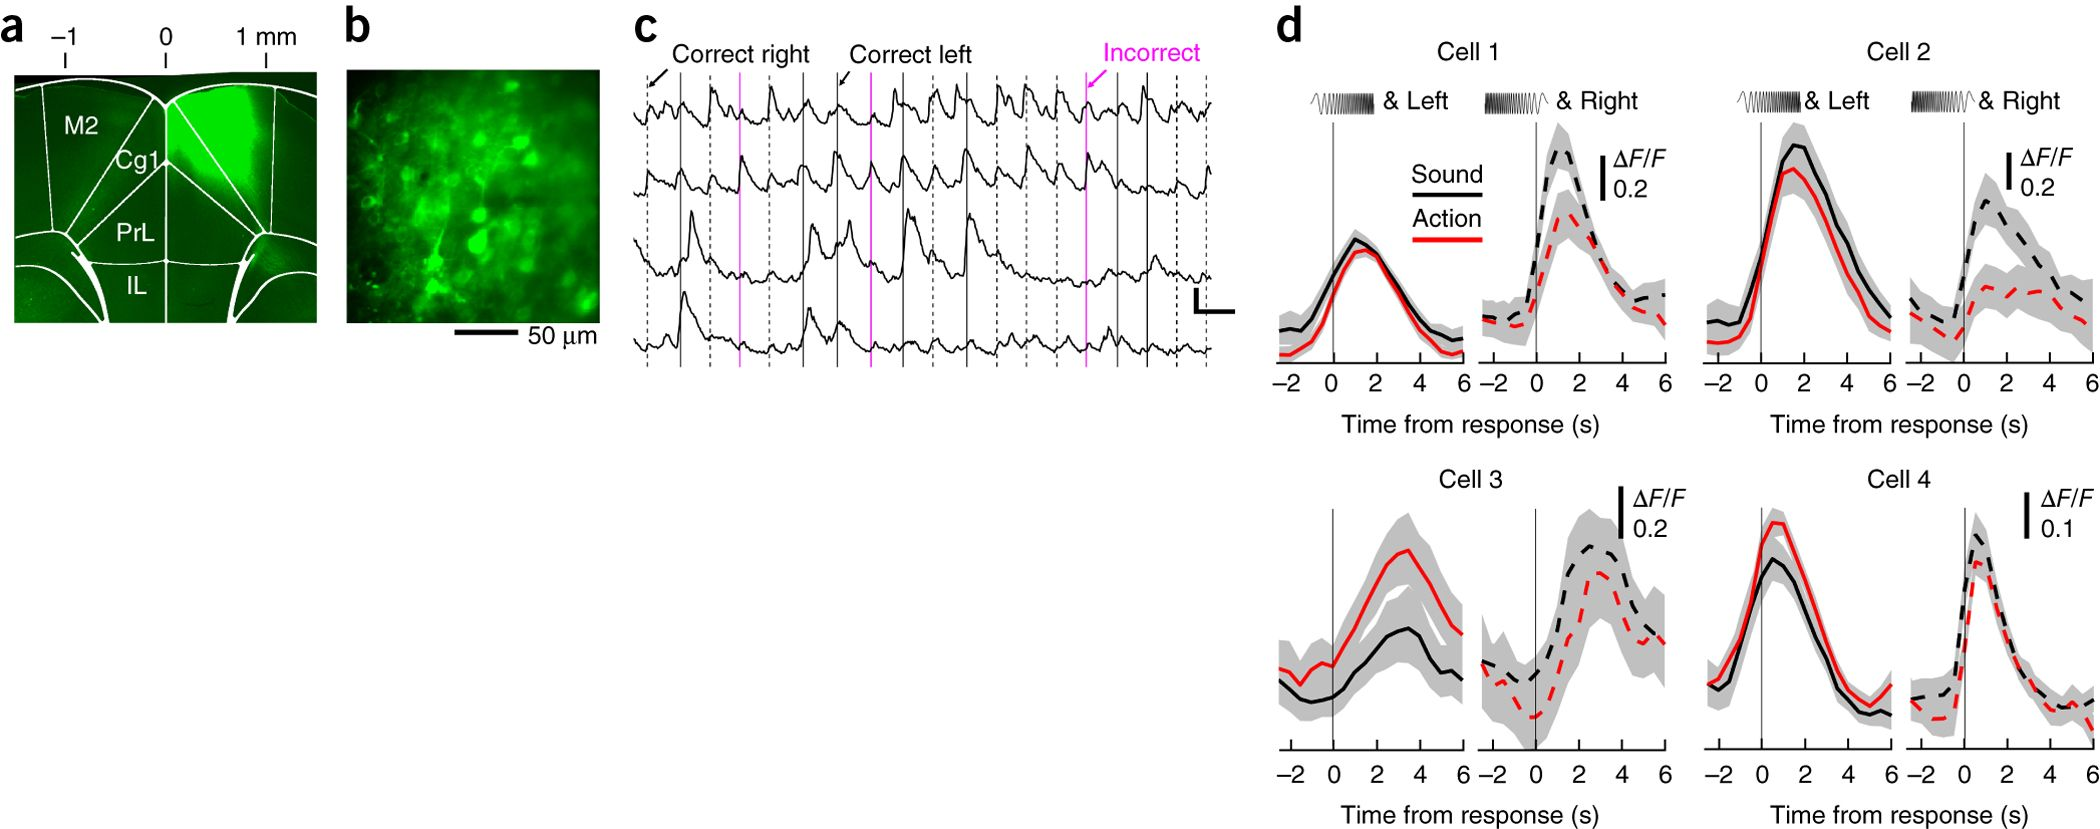
\includegraphics[width=\textwidth]{Figures/Chapter3/NN_fig3} 
\end{center}

\caption[Two-photon Ca$^{2+}$ imaging of task-related activity in M2]
{
Two-photon calcium imaging of task-related activity in M2.
(a) Example post hoc and (b) \emph{in vivo} two-photon images of GCaMP6s-expressing neurons in layer 2/3 of M2. PrL, prelimbic cortex; IL, infralimbic cortex. (c) Fractional fluorescence changes ($\Delta F/F$) in example M2 neurons during performance of sound-guided trials. Vertical lines indicate the time of response associated with correct left (solid black), correct right (dotted black), or incorrect (magenta) trials. Scale bars, 10 s and 100\% $\Delta F/F$. (d) Trial-averaged $\Delta F/F$ of four M2 neurons for correct left (solid line) and correct right (dotted line) responses in sound-guided (black) and action-guided (red) trials. Cell 1 corresponds to the top trace in c. Lines, mean. Gray shading, 95\% confidence intervals.
}


\label{fig:NN_fig3}
\end{figure}